\documentclass[a4paper,10pt]{article}

% Hier die Nummer des Blatts und Autoren angeben.
\newcommand{\blatt}{1}
\newcommand{\autor}{Brigitte Kwasny}

\usepackage{hci}

\begin{document}
% Seitenkopf mit Informationen
\kopf
\renewcommand{\figurename}{Figure}

\tableofcontents

\part{Organisatorisches}

\section{Ziele der Vorlesung}
\begin{enumerate}
\item Entwurf, Aufbau und Wartung von Datenbanken, insbesondere auf der Basis
\item Sicherung der Ablaeufe auf Datenbanken \emph{(Transaktionsprogramme)}
\item Verwaltung und Handhabung semi-strukturierter Daten/Dokumente (XML)
\item Entwicklung von (betrieblichen) Anwendungs- und Informationssystemen, insb. datenbankgestuetzter Anwendungen
\item Nutzung (semi-)strukturierter Datenquellen unter Verwendung spezifischer Sprachansaetze
\item Systemverantwortlicher fuer Informations- und Datenbanksysteme, insbesondere Unternehmens-, Datenbank-, Anwendungs- und Datensicherungsadministrator
\end{enumerate}

\section{Klausur}
Die Klausur findet am 09.02.2017 von 12:30 - 14:30 Uhr im Audimax statt.

\newpage
\part{Vorlesung 1}
Heute werden wir von einer elektronischen Informationsflut ''ueberrollt'', deshalb gewinnen \textbf{Datenbankverwaltungssysteme} (DBMS - \emph{database management systems}) eine immer groessere Bedeutung.\\
Ein DBMS besteht aus einer Menge von \textbf{Daten} und den zur Datenverarbeitung notwendigen Programmen:
\begin{enumerate}
\item Die gespeicherten Daten werden oft als \textbf{Datenbasis} bezeichnet =\textgreater enthaelt die miteinander in Beziehung stehenden Informationseinheiten, die zur Kontrolle und Steuerung eines Aufgabenbereichs (evtl. eines ganzen Unternehmens) notwendig sind
\item Die Gesamtheit der Programme zum Zugriff auf die Datenbasis, zur Kontrolle der Konsistenz und zur Modifikation der Daten wird als \textbf{Datenbankverwaltungssystem} bezeichnet
\end{enumerate}
Oft werden diese Komponenten weniger scharf getrennt, sodass ein DBMS in der Regel beides meint.

\section{Motivation, Einfuehrung und Grundbegriffe}

\subsection{Motivation}
\subsubsection{Motivation (1)}
\textbf{Betriebliche Informationssysteme und E-Business}\\
Betriebliche Informationssysteme spiegeln die Geschaeftsmodelle von Unternehmen wider und dienen dazu, deren Arbeitslaeufe zu organisieren und zu unterstuetzen; sie sind \textbf{stark datenbankbasierte Anwendungen} mit \textbf{vielen Benutzern} und \textbf{transaktionsverarbeitende Systeme}. Dabei muss die \textbf{Integritaet der Daten} gewaehrleistet sein, sowie \textbf{hohen Durchsatz und kurze Antwortzeiten} muessen geschaffen werden. Sie sind \textbf{nicht nur Dialogsysteme}, sondern benoetigen meist einen \textbf{Batch}.

\subsubsection{Motivation (2)}
E-Business ist die Nutzung des Internets zu geschaeftlichen Zwecken aller Art. Bei E-Commerce fliesst Geld, denn es geht um Handel, also den Abschluss und die Abwicklung von Kaufvertraegen. Dabei werden Varianten unterschieden, je nachdem, wer mit wem handelt:\\
ein Unternehmen mit seinen Endkunden \emph{(Business-to-Consumer, B2C)}, Unternehmen untereinander \emph{(Business-to-Business, B2B)} oder Endkunden direkt miteinander ueber Boersen und Auktionen \emph{(Consumer-to-Consumer, C2C)}.

\subsubsection{Motivation (3)}
E-Business braucht starke Softwaresysteme. Es sind \textbf{komplexe Systeme}, denn es genuegt nicht, sich mit einer gut gestalteten Web-Oberflaeche dem Benutzer zu praesentieren - werblich ansprechend, um ihn zu gewinnen; ergonomisch, um ihn nicht zu verlieren.\\
Dahinter muss mehr stehen: \textbf{eine flexible Anwendung}, die sich schnell an geaenderte Geschaeftsprozesse anpassen laesst, und eine \textbf{gehaltvolle Datenbank}.\\
E-Business-Systeme sind \textbf{eigentlich ueberbetriebliche Informationssysteme}, denn sie \textbf{verbinden} ueber ein Unternehmen hinausgehend Mitarbeiter, Lieferanten und Kunden und werden vor allem von Menschen genutzt.

\subsubsection{Motivation (4)}
Man muss eine noch nie da gewesene \textbf{Komplexitaet der Technologie} beherrschen. Man muss sich mit der \textbf{Programmierung der Web-Oberflaeche} auskennen \emph{(HTML, XML, Java-Applets)}, \textbf{Netzprotokolle} \emph{(z.B. HTTP)} und \textbf{Web-Server} einzusetzen verstehen, \textbf{Anwendungsprogramme in Java} schreiben und unter der \textbf{Transaktionskontrolle} von \textbf{Application-Servern} zum Laufen bringen.\\
Standard-Internet-Anwendungen \emph{(z.B. Intershop)} sowie vorhandene (Legacy-)Systeme integrieren.

\subsection{Miniwelt}
Ein Datenbanksystem \textbf{verwaltet Daten} einer realen oder gedanklichen Anwendungswelt. Diese Daten gehen aus Informationen hervor, die stets aus den Sachverhalten und Vorgaengen dieser Anwendungswelt \textbf{durch gedankliche Abstraktionen} gewonnen werden.\\
Sie beziehen sich nur auf solche Aspekte des betrachteten Weltausschnitts, die fuer den Zweck der Anwendung relevant sind. Ein solcher Weltausschnitt wird auch als \textbf{Miniwelt} \emph{(Diskurswelt)} bezeichnet.
\\~\\
TODO

\subsection{Informationssystem}
\textbf{Definitionen nach Hansen:}
\begin{enumerate}
\item Ein \textbf{Informationssystem (IS)} besteht aus Menschen und Maschinen, die Informationen erzeugen und/oder benutzen und die durch Kommunikationsbeziehungen miteinander verbunden sind
\item Ein \textbf{betriebliches IS} dient zur Abbildung der Leistungsprozesse und Austauschbeziehungen im Betrieb und zwischen dem Betrieb und seiner Umwelt
\item Ein \textbf{rechnergestuetztes IS} ist ein System, bei dem die Erfassung, Speicherung und/oder Transformation von Informationen durch den Einsatz von EDV \textbf{teilweise automatisiert} ist =\textgreater KIS \emph{(kooperatives Informationssystem)} besteht aus einer Menge unabhaengiger Systeme, die zusammen die angestrebte Leistung erbringen
\end{enumerate}

\begin{enumerate}
\item Eine \textbf{Datenbank (DB)}
\begin{itemize}
\item ist eine Sammlung gespeicherter operationaler Daten, die von den Anwendungssystemen eines Unternehmens benoetigt werden
\end{itemize}
\item Ein \textbf{Datenbankverwaltungssystem (DBVS)}
\begin{itemize}
\item ist ein standardisiertes Softwaresystem zur Definition, Verwaltung, Verarbeitung und Auswertung der DB-Daten
-item kann mittels geeigneter Parametrisierung an die speziellen Anwendungsbeduerfnissen angepasst werden \emph{(hochgradig generisches System)}
\item implementiert ein \textbf{Datenmodell}, das die Art der Datenstrukturen und generische Operationen zu deren Manipulation bereitstellt
\end{itemize}
\item Ein \textbf{Datenbanksystem (DBS)}
\begin{itemize}
\item TODO
\end{itemize}
\end{enumerate}

\subsection{Zusammenfassung}
\textbf{Daten:} objektive Welt der nicht-interpretierten Daten\\
\textbf{Information:} subjektive Welt der bewerteten Daten\\
\textbf{grob:} $DB + DBVS = DBS$; $DBS + AWS = KIS$\\
\textbf{=\textgreater} Heterogenitaet, Wachstum, Anforderungsvielfalt u.a. fuehren oft zu unabhaengigen IS, die zusammen als kooperatives IS die angestrebte Leistung erbringen muessen
\\~\\
Beispiele zu verschiedenen Informationssystemen: Universitaet, Produktionsbetriebes, Fluggesellschaft, Bank etc.

\newpage
\section{Anforderungen und (Schichten-)Modelle}
Schichtenmodelle auch als \textbf{Beschreibungsmodell} bezeichnet.

\subsection{Nutzung von Dateisystemen}
\textbf{Dateisystem:}
\begin{enumerate}
\item permanente Datenhaltung innerhalb von Betriebssystem-Dateien
\item Betriebs/Dateisystem bietet Funktionen fuer die \textbf{Erzeugung / Loeschen} von Dateien, \textbf{Zugriffsmoeglichkeiten} auf Bloecke/Saetze der Datei und \textbf{einfache Operationen} zum Lesen/Aendern/Einfuegen/Loeschen von Saetzen
\end{enumerate}

Daten auf Papier oder in isolierten Computer-Dateien abzulegen fuehrt meist zu folgenden schwerwiegenden Problemen:
\begin{enumerate}
\item \textbf{Redundanz und Inkonsistenz}
\begin{itemize}
\item Bei Aenderungen von redundanten Daten kann dies zu Inkonsistenzen fuehren, wenn nur eine Kopie der Daten geaendert wird, die andere aber noch im vealteten Zustand beibehalten wird
\end{itemize}
\item \textbf{Beschraenkte Zugriffsmoeglichkeiten}
\begin{itemize}
\item die in isolierten Dateien abgelegten Daten kann man unmoeglich miteinander ''verknuepfen''
\end{itemize}
\item \textbf{Probleme des Mehrbenutzerbetriebs}
\begin{itemize}
\item Die heutigen Dateisysteme bieten entweder gar keine oder nur sehr rudimentaere Kontrollmechanismen fuer den Mehrbenutzerbetrieb. Daten werden i.A. von sehr vielen Anwendern innerhalb und ausserhalb der jeweiligen Organisation genutzt \emph{(z.B. Flugreservierungssystem)}. \textbf{Bei unkontrolliertem Zugriff} kann es sehr leicht zu unerwuenschten Anomalien kommen \emph{(z.B. Gleichzeitiges Editieren desselben Datensatzes durch zwei Benutzer)} =\textgreater \textbf{''lost update''}
\end{itemize}
\item \textbf{Verlust von Daten}
\begin{itemize}
\item Wenn Daten in isolierten Dateien gehalten werden, wird die Wiederherstellung eines konsistenten - d.h. eines gemaess der realen Welt gueltigen Zustands der Gesamtinformationsmenge im Fehlerfall sehr schwierig. Im Allgemeinen bieten Dateisysteme bestenfalls die Moeglichkeit einer periodisch durchgefuehrten Sicherung der Dateien. \textbf{Datenverluste}, die waehrend der Bearbeitung von Dateien oder nach der letzten Sicherungskopie auftreten, sind i.A. nicht auszuschliessen
\end{itemize}
\item \textbf{Integritaetsverletzung}
\begin{itemize}
\item Je nach Anwendungsgebiet gibt es vielfaeltigste, sich global ueber mehrere Informationseinheiten erstreckende Integritaetsbedingungen \emph{(z.B. Stundenten muessen erst die Pflichtseminare abgeschlossen haben, bevor sie zur Pruefung zugelassen werden oder max zwei Pruefungsversuche)}. Die Einhaltung derartiger Integritaetsbedingungen ist bei der isolierten Speicherung der Informationseinheiten in verschiedenen Dateien sehr schwierig, da man zur Kontrolle Daten aus unterschiedlichen Dateien verknuepfen muss \emph{(siehe oben)}. Ausserdem will man im Allgemeinen nicht nur die \textbf{Konsistenzbedingungen} ueberpruefen, sondern die \textbf{Einhaltung erzwingen}
\end{itemize}
\item \textbf{Sicherheitsprobleme}
\begin{itemize}
\item Nicht alle Benutzer sollten Zugriff auf die gesamten gespeicherten Daten haben. Und erst recht sollten nur bestimmte ausgewaehlte Benutzer das \textbf{Privileg zum Editieren} haben
\end{itemize}
\item \textbf{Hohe Entwicklungskosten}
\begin{itemize}
\item In vielen Faellen muss fuer die Entwicklung eines neuen Anwendungsprogrammes praktisch ''das Rad neu erfunden'' werden. Jedesmal muss sich der Anwendungsprogrammierer zusaetzlich zu Fragen der Dateiverwaltung mit zumindest einer Teilmenge der obigen Probleme auseinandersetzen.
\end{itemize}
\end{enumerate}
Alle Probleme, die hier aufgezaehlt wurden, werden durch ein DBMS abgeloest, da es interne Moeglichkeiten fuer die Realisierung bietet.

\subsection{Datenabstraktion / Schema-Architektur (Folie)}
Man unterscheidet drei Abstraktionsebenen \emph{(ANSI-SPARC-Architektur oder auch Drei-Schema-Architektur)} im Datenbanksystem:
\begin{enumerate}
\item \textbf{Die physische / interne Ebene}
\begin{itemize}
\item Auf dieser Ebene wird festgelegt, wie die Daten gespeichert sind. Im Allgemeinen sind Daten auf dem Hintergrundspeicher \emph{(Festplatte)} abgelegt
\end{itemize}
\item \textbf{Die logische / konzeptionelle Ebene}
\begin{itemize}
\item Auf der logischen Ebene wird in einem sogenannten \textbf{Datenbankschema} festgelegt, welche Daten abgespeichert werden
\end{itemize}
\item \textbf{Die Sichten / Externe Ebene}
\begin{itemize}
\item Waehrend das Datenbankschema der logischen Ebene ein integriertes Modell der gesamten Informationsmenge des jeweiligen Anwendungsbereichs darstellt, werden \textbf{in den Sichten} Teilmengen der Information bereitgestellt =\textgreater Die Sichten sind \textbf{auf die Beduerfnisse} der jeweiligen Benutzer(-gruppen) zugeschnitten \emph{(z.B. drei Studenten, die Professoren oder der Hausmeister)} =\textgreater Zugriffsschutz, Reduktion der Komplexitaet
\end{itemize}
\end{enumerate}
Zum einen wollen Anwender i.A. nur einen Ausschnitt des gesamten Informationsmodells zu sehen bekommen. Zum anderen koennen bestimmte kritische Informationsteile in den Sichten ausgeblendet werden, um dadurch den Datenschutz zu gewaehrleisten.

\begin{figure}
    \centering
    \includegraphics[width=0.9\textwidth]{images/Drei-Ebenen-Schema-Architektur.png}
\end{figure}	

\subsection{Datenunabhaengigkeit}
\emph{nicht in VL erwaehnt}
\\~\\
Die drei Ebenen eines DBMS gewaehrleisten einen bestimmten Grad der \textbf{Datenunabhaengigkeit}. Dies ist analog zum Konzept der \textbf{abstrakten Datentypen} (ADTs) in Programmiersprachen. Durch eine wohldefinierte Schnittstelle wird die ''darunterliegende'' Implementierung verdeckt, so dass man - bei Beibehaltung der Schnittstelle - die Realisierung variieren kann, ohne dass die Benutzer der Schnittstelle davon in Mitleidenschaft gezogen werden.
\\~\\
Aufgrund der drei Schichten ergeben sich zwei Stufen der Datenunabhaengigkeit im DBMS:
\begin{enumerate}
\item \textbf{Physische Datenunabhaengigkeit}
\begin{itemize}
\item TODO
\end{itemize}
\item \textbf{Logische Datenunabhaengigkeit}
\begin{itemize}
\item TODO
\end{itemize}
\end{enumerate}

Die heutigen Datenbanksysteme erfuellen zumeist die physische Datenunabhaengigkeit. Die logische Datenunabhaengigkeit kann schon rein konzeptuell nur fuer einfachste Modifikationen des Datenbankschemas gewaehrleistet sein.

\subsection{Grundbegriffe}
\textbf{Datenbank (DB)} als \textbf{Abbildung einer Miniwelt}
\begin{enumerate}
\item Vorgaenge und Sachverhalte werden als gedankliche Abstraktionen der Miniwelt erfasst und als Daten \textbf{in} der Datenbank gespeichert
\item Daten beziehen sich nur auf solche Aspekte der Miniwelt, die fuer die Zwecke der Anwendung relevant sind
\item Eine DB ist integritaetserhaltend (bedeutungstreu), wenn ihre Objekte Modelle einer gegebenen Miniwelt repraesentieren
\end{enumerate}

\textbf{Datenmodell, DB-Schema und DB-Instanz}\\
Datenbankverwaltungssysteme basieren auf einem \textbf{Datenmodell}, das sozusagen die Infrastruktur fuer die Modellierung der realen Welt zur Verfuegung stellt. Das Datenmodell legt die Modellierungskonstrukte fest, mittels derer man ein computerisiertes Informationsabbild der realen Welt \emph{(bzw. des relevanten Ausschnitts)} generieren kann.
\begin{enumerate}
\item Datenmodell legen Regeln fest, nach denen die Objekte von DBs erzeugt und veraendert werden
\item DB-Schema legt die Auspraegungen der Objekte fest, welche die DB fuer eine bestimmte Miniwelt einnehmen kann
\item DB-Instanz entspricht tatsaechlicher (schema-konformer) Auspraegung einer Menge von Objekten
\end{enumerate}
Das Datenmodell ist somit analog zu einer Programmiersprache: Es legt die generischen Strukturen und Operatoren fest, die man zur Modellierung einer bestimmten Anwendung ausnutzen kann. Eine Programmiersprache legt die Typkonstruktoren und Sprachkonstrukte fest, mit deren Hilfe man spezifische Anwendungsprogramme realisiert.
\\~\\
Das Datenmodell besteht demnach aus zwei Teilsprachen:
\begin{enumerate}
\item der \textbf{Definitionssprache} \emph{(DDL - data definition language)}
\item der \textbf{Datenmanipulationssprache} \emph{(DML - data manipulation language)}
\end{enumerate}
Die DDL wird benutzt, um die Struktur der abzuspeichernden Datenobjekte zu beschreiben. Dabei werden gleichartige Datenobjekte durch ein gemeinsames Schema \emph{(analog zu einem Datentyp in Programmiersprachen)} beschrieben. Die Strukturbeschreibung aller Datenobjekte des betrachteten Anwendungsbereichs nennt man das \textbf{Datenbankschema}.
\\~\\
Die Datenmanipulationssprache besteht aus
\begin{itemize}
\item der \textbf{Anfragesprache} \emph{(Query Language)} und
\item der ''eigentlichen'' Datenmanipulationssprache zur Aenderung von abgespeicherten Daten und zum Loeschen von gespeicherten Daten
\end{itemize}

Die DML (inkl. Anfragesprache) kann in zwei unterschiedlichen Arten genutzt werden:
\begin{itemize}
\item \textbf{interaktiv}, TODO
\item TODO
\end{itemize}

\textbf{Beschreibung und Handhabung der Daten}
\begin{enumerate}
\item Daten muessen interpretierbar sein
\item Daten muessen bei allen am Austausch beteiligten Partnern (Systemen, Komponenten) die Ableitung derselben Information erlauben
\item Einsatzspektrum verlangt generische Vorgehensweise
\begin{enumerate}
\item Beschreibung der zulaessigen DB-Zustaende
\item Beschreibung der zulaessigen Zustandsuebergaenge (generische Operatoren)
\end{enumerate}
\end{enumerate}

\textbf{Anwendungsprogrammier-Schnittstelle (API)}
\begin{enumerate}
\item Operatoren zur Definition von Objekttypen \emph{(Beschreibung der Objekte)}
\begin{enumerate}
\item \textbf{DB-Schema:} Welche Objekte sollen in der DB gespeichert werden?
\end{enumerate}
\item Operatoren zum Aufsuchen und Veraendern von Daten
\begin{enumerate}
\item \textbf{AW-Schnittstelle:} Wie erzeugt, aktualisiert und findet man DB-Objekte?
\end{enumerate}
\item Operatoren zur Definition von Integritaetsbedingungen \emph{(Constraints)}
\begin{enumerate}
\item \textbf{Sicherung der Qualitaet:} Was ist ein akzeptabler DB-Zustand?
\end{enumerate}
\item Operatoren zur Definition von Zugriffskontrollbedingungen
\begin{enumerate}
\item \textbf{Massnahmen zum Datenschutz:} Wer darf was?
\end{enumerate}
\end{enumerate}

\subsection{Datenbankschema und Auspraegung}
\emph{nicht in VL erwaehnt}
\\~\\
TODO

\subsection{Einordnung der Datenmodelle}
\emph{nicht in VL erwaehnt}
\\~\\
In Abbildung 1.2 sind die grundlegendsten Phasen der Datenmodellierung gezeigt.
\\~\\
\textbf{Modelle des konzeptuellen Entwurfs}\\
Man beginnt beim Datenbankentwurf mit der Abgrenzung eines Teils der ''realen Welt'', um den Ausschnitt \emph{(Miniwelt)} zu bestimmen, der in der Datenbank modelliert werden soll. Diese Miniwelt wird dann konzeptuell modelliert.
\\~\\
Fuer die konzeptuelle Modellierung gibt es mehrere moegliche Datenmodelle:
\begin{enumerate}
\item Entity-Relationship-Modell \emph{(auch Gegenstand-Beziehungs-Modell)}
\item semantisches Datenmodell
\item objektorientierte Entwurfsmodelle \emph{(wie UML)}
\end{enumerate}

\subsection{Anforderungen an ein DBS}
\begin{enumerate}
\item \textbf{Kontrolle ueber die operationalen Daten}
\item \textbf{Leichte Handhabbarkeit der Daten}
\item \textbf{Kontrolle der Datenintegritaet}
\item \textbf{Leistung und Skalierbarkeit}
\item \textbf{Hoher Grad an Daten-Unabhaengigkeit}
\end{enumerate}

TODO

\subsection{Schichtenmodell fuer DBS}
TODO

\subsection{Dynamischer Ablauf einer DB-Operation}
\begin{lstlisting}[language=SQL]
SELECT * FROM `person` WHERE pnr = `12345`
\end{lstlisting}

\begin{enumerate}
\item Vervollstaendigen der Verarbeitungsinformation aus Konzeptionellem und Internem Schema
\begin{enumerate}
\item Ermittlung der Seiten \emph{(z.B. durch Hashing)}
\end{enumerate}
\item Zugriff auf DB-Puffer: falls erfolgreich, dann weiter mit 7
\item Zugriff auf DB ueber DB-Pufferverwaltung/Betriebssystem
\item Durchfuehrung des E/A-Auftrages
\item Ablegen der Seite im DB-Puffer
\item Uebertragen des Anfrageergebnisses in den Arbeitsbereich der Anwendung
\item Statusinformation: Return-Code, Cursor-Info
\item Manipulation mit Anweisungen der Programmiersprache
\end{enumerate}

\subsection{Zusammenfassung}
\textbf{DBS-Charakteristika:}\\
\textbf{Zentralisierte Verwaltung} der operationalen Daten \emph{(Rolle des DBA)}, Adaequate Schnittstellen \emph{(Datenmodell und DB-Sprache)}, Datenkontrolle - insb. zentrale Kontrolle der Datenintegritaet und kontrollierter Mehrbenutzerbetrieb, Leistung und Skalierbarkeit, Hoher Grad an Daten-Unabhaengigkeit
\\~\\
\textbf{Beschreibungsmodelle fuer ein DBS:}\\
Schichtenmodell, Drei-Schema-Architektur
\\~\\
\textbf{Programmierschnittstellen:} \emph{(siehe Schichtenmodell)}\\
mengenorientierte DB-Schnittstelle \emph{(relationale DBS)}, satzorientierte DB-Schnittstelle \emph{(hierarchische und netzwerkartige DBS)}, interne Satzschnittstelle \emph{(zugriffsmethodenorientierte Programmierschnittstelle)}

\section{Zusammenfassung: Vorlesung 1}
TODO

\newpage
\part*{Vorlesung 2}
Das mit Abstand am haeufigsten benutzte Modell fuer den konzeptuellen Entwurf ist das \textbf{Entity-Relationship-Modell}. In der konzeptuellen Entwurfsphase werden die in der realen Welt vorkommenden Konzepte in Gegenstandsmengen und Beziehungen zwischen diesen Gegenstandsmengen strukturiert.
\\~\\
Abbildung 1.3 zeigt diese ''intellektuelle'' Aufgabe fuer einen ganz kleinen Ausschnitt der Universitaetswelt. Es werden die Gegenstandsmengen \emph{Studenten, Professoren} und \emph{Vorlesungen} ermittelt. Weiterhin werden die Beziehungen \emph{hoeren} und \emph{lesen} bestimmt.
\\~\\
Die konzeptuellen Datenmodelle verfuegen im Allgemeinen nur ueber eine DDL und haben keine Datenmanipulationssprache, da sie nur die Struktur der Daten beschreiben. Sie verzichten auf die Abbildung von individuellen Datenobjekten, d.h. es werden keine Datenbankauspraegungen erzeugt. Deshalb benoetigen sie keine Datenmodifikationssprache (DML).

\section{Informationsmodellierung}

\subsection{DB-Entwurf und Modellierung}
\textbf{Ziel:} Modellierung einer Miniwelt: modellhafte Abbildung eines anwendungsorientierten Ausschnitts der realen Welt (Miniwelt) und Nachbildung von Vorgaengen durch \textbf{Transaktionen}\\
\textbf{Nebenbedingungen:} genaue Abbildung, hoher Grad an Aktualitaet, Verstaendlichkeit, Natuerlichkeit, Einfachheit\\
\textbf{Zwischenziel:} Erhebung der Information in der Systemanalyse (Informationsbedarf), \textbf{Informationsmodell} (allg. Systemmodell)\\
\textbf{Bestandteile:} Objekte: Entities, Beziehungen: Relationships
\\~\\
\textbf{Informationsmodell:} Darstellungselemente und Regeln, eine Art formale Sprache, um Informationen zu beschreiben\\
\textbf{Informationen ueber Objekte und Beziehungen nur, wenn:} unterscheid- und identifizierbar, relevant und selektiv beschreibbar

\subsection{Entity-Relationship-Modell}
\textbf{Modellierungskonzepte:} Entity-Mengen (Objektmengen), Wertebereiche, Attribute, Primaerschluessel, Relationship-Mengen (Beziehungsmengen)\\
\textbf{Klassifikation der Beziehungstypen:} benutzerdefinierte Beziehungen, Abbildungstyp \emph{($1:1$, $1:n$, $n:m$)}\\
=\textgreater \textbf{Ziel:} Festlegung von semantischen Aspekten, explizite Definition von strukturellen Integritaetsbedingungen
\\~\\
\textbf{(!)} Das ERM modelliert die \textbf{Typ-}, nicht die Instanz\textbf{ebene}; es macht also Aussagen ueber Entity- und Relationship-Mengen, nicht jedoch ueber einzelne ihrer Elemente (Auspraegungen). Die Modellierungskonzepte des ERM sind haeufig zu ungenau oder unvollstaendig. Sie \textbf{muessen} deshalb \textbf{ergaenzt werden} durch \textbf{Integritaetsbedingungen} (Constraints).

\subsubsection{Entity}
Entities sind wohlunterscheidbare Dinge der Miniwelt (Diskurswelt) und besitzen Eigenschaften, deren konkrete Auspraegungen als Werte bezeichnet werden.
\\~\\
\textbf{Entity-Mengen}: Zusammenfassung von ''aehnlichen'' oder ''vergleichbaren'' Entities und haben gemeinsasme Eigenschaften\\
=\textgreater Bsp: Abteilungen, Angestellte, Projekte ... / Buecher, Autoren, Leser ...
\\~\\
\textbf{Wertebereiche und Attribute:} \textbf{(1)} Die moeglichen oder ''zulaessigen'' Werte fuer eine Eigenschaft nennen wir Wertebereich (oder Domain). \textbf{(2)} Die (bei allen Entities einer Entity-Menge auftretenden) Eigenschaften werden als Attribute bezeichnet und \textbf{(3)} ein Attribut ordnet jedem Entity einer Entity-Menge einen Wert aus einem bestimmten Wertebereich (dem des Attributs) zu.

\subsubsection{Beispiel: ''Buch'' (Entity-Typ)}
PICTURE in Folie

\begin{itemize}
\item jedem Attribut ist einem geeignetem Wertebereich zugeordnet
\item Name der Entity-Menge sowie die zugehoerigen Attribute sind \textbf{zeitinvariant}
\item Entity-Menge und ihre Entities sind \textbf{zeitveraenderlich}
\end{itemize}

PICTURE in Folie

\textbf{Erhoehung der Modellierungsgenauigkeit} durch
\begin{itemize}
\item einwertige Attribute
\item mehrwertige Attribute (Doppelovale)
\item zusammengesetzte Attribute (hierarchisch angeordnete Ovale)
\item Verschachtelungen sind moeglich
\end{itemize}

\subsubsection{Wie wird ein Entity identifiziert?}
Entities muessen ''wohlunterscheibar'' sein und die Information ueber ein Entity ist ausschliesslich durch den (Attribut-)Wert definiert.\\
\textbf{Identifikation} eines Entities durch Attribut:
\begin{itemize}
\item $1:1$ Beziehung (ggf. kuenstlich erzwungen durch laufende Nummer)
\end{itemize}

TODO mit Formeln

\subsubsection{Definition: Entity-Typ}
Ein Entity-Typ hat die Form $E = (X, K)$ mit einem Namen $E$, einem Format $X$ und einem Primaerschluessel $K$, der aus (einwertigen) Elementen von $X$ besteht. Die Elemente eines Formats $X$ werden dabei wie folgt beschrieben:
\begin{itemize}
\item einwertige Attribute $A$
\item mehrwertige Attribute ${A}$
\item zusammengesetzte Attribute $A (B_1, ..., B_k)$
\end{itemize}

\subsubsection{Definition: Wertebereich / Domain}
Sei $E = (X, K)$ ein Entity-Typ und $attr(E)$ die Menge aller in $X$ vorkommenen Attributnamen. Jedem $A \in attr(E)$, das nicht einer Zusammensetzung voransteht, sei ein Wertebereich $W(A)$ zugeordnet. Fuer jedes $A \in attr(E)$ sei
\begin{itemize}
\item $dom(A) := W(A)$, falls $A$ einwertig
\item $dom(A) := 2^{W(A)}$, falls $A$ mehrwertig
\item $dom(A) := W(B_1) x ... x W(B?k)$, falls $A$ aus einwertigen $B_1, ..., B_k$ zusammengesetzt
\end{itemize}
Besteht $A$ aus mehrwertigen oder zusammengesetzten Attributen, wird die Definition rekursiv angewendet.

\subsubsection{Definition: Entity und Entity-Menge}
Sei $E = (X, K)$ ein Entity-Typ mit $X = (A_1, ..., A_m)$. $A_i$ sei $dom(A_i) (1 \leq i \leq m)$ zugeordnet.
\begin{itemize}
\item Ein Entity $e$ ist ein Element des Kartesischen Produkts aller Domains, d.h. $e \in dom(A_1) x ... x dom(A_m)$
\item Eine Entity-Menge $E^{t}$ (zum Zeitpunkt $t$) ist eine Menge von Entities, welche K erfuellt, d.h. $E^{t} \subseteq dom(A_1) x ... x dom(A_m)$
\end{itemize}
$E^{t}$ wird auch als der Inhalt bzw. der aktuelle Wert (Instanz) des Typs $E$ zur Zeit $t$ berechnet.

\subsubsection{Definition Relationship, Relationship-Typ und Relationship-Menge}
Ein Relationship-Typ hat die Form $R = (Ent, Y)$. Dabei ist $R$ der Name des Typs, $Ent$ bezeichnet die Folge der Namen der Entity-Typen, zwischen denen die Beziehung definiert ist und $Y$ ist eine (moeglicherweise leere) Folge von Attributen der Beziehung.
\\~\\
Sei $Ent = (E_1, ..., E_k)$ und fuer ein beliebiges, aber festes $t$ sei ${E_i}^t$ der Inhalt des Entity-Typs $E_i$, $1 \leq i \leq k$. Ferner sei $Y = (B_1, ..., B_n)$. Ein Relationship $r$ ist ein Element des Kartesischen Produktes aus allen ${E_i}^t$ und den Domains der $B_j$, d.h.
\begin{itemize}
\item $r \in {E_i}^t x ... x {E_i}^t x dom(B_1) x ... x dom(B_n)$ bzw
\item $r = (e_1, ..., e_k, b_1, ..., b_n)$ mit
\item $e_i \in {E_i}^t$ fuer $1 \leq i \leq k$ und $b_j \in dom(B_j)$ fuer $1 \leq j \leq n$
\end{itemize}

Eine Relationship-Menge $R^t$ (zur Zeit t) ist eine Menge von Relationships, d.h.
\begin{itemize}
\item $R^t \subseteq {E_i}^t x ... x {E_i}^t x dom(B_1) x ... x dom(B_n)$
\end{itemize}

\textbf{Eigenschaften von Relationship-Mengen:}
Grad $n$ der Beziehung \emph{(degree)}, gewoehnlich $n = 2$ oder $n = 3$, Existenzabhaengigkeit, Beziehungstyp \emph{(connectivity)} und Kardinalitaet
\\~\\
PICTURE von Folie
\\
Ausleihe = ((Leser, Buch), (RDatum))\\
\textbf{Eigenschaften:} Grad = 2, Existenzabhaengigkeit = false, Beziehungstyp = $n:m$

\subsubsection{Beispiele}
TODO

\subsection{Erweiterungen des ERM}
TODO

\subsection{Zusammenfassung}
\textbf{DB-Entwurf umfasst:} \textbf{(1)} Informationsbedarfsanalyse, \textbf{(2)} konzeptionelles DB-Schema (-\textgreater Informationsmodell), \textbf{(3)} logisches DB-Schema \emph{(nicht diskutiert)}, \textbf{(4)} physisches DB-Schema \emph{(nicht diskutiert)}
\\~\\
\textbf{ERM-Charakteristika:} \textbf{(1)} Modellierung bezieht sich auf die Typeebene, \textbf{(2)} relevante Zusammenhaenge der Miniwelt werden durch Entity- und Relationship-Mengen modelliert; sie werden genauer durch Attribute, Wertebereiche, Primaerschluessel/Schluesselkandidaten beschrieben, \textbf{(3)} Klassifikation von Beziehungstypen dient der Spezifikation von strukturellen Integritaetsbedingungen, \textbf{(4)} anschauliche Entwurfsdarstellung durch ER-Diagramme und \textbf{(5)} relativ karges Informationsmodell
\\~\\
\textbf{Einfuehrung weiterer Modellierungskonzepte:} TODO


\newpage
\part*{Vorlesung 3}
\section{Grundlagen des Relationenmodells}

\section{Die Standardsprache SQL}

\section{Logischer DB-Entwurf}

\section{Transaktionsverwaltung, Integritaetssicherung und Zugriffskontrolle}

\section{DB-Zugriffsverfahren}

\section{Semistrukturierte Daten und XML}

\end{document}